\section{Program Decomposition} \label{sec:decompose}
The output of the previous step (\Cref{sec:control}) is a VBDFG that correctly executes the original program on an RDA without resource constraint. 
The {\em PB allocation} phase enforces and addresses constraint violations given a hardware specification of the RDA. 
In the end, each VB is assigned to a PB type used by PaR to map VBs onto the actual PBs.

In contrast to a combined VB allocation and assignment approach, where each VB is allocated for a specific type of PB, our approach enables maximum resource utilization with specialization in PBs, because we model what resource each VB consumes and each PB processes without tracking what types they are.
For example, an application without DRAM access can use the specialized DRAM address generator PB to perform other computations.

To enforce resource constraints, \name{} uses a VB-PB bipartite graph to keep track of potential valid assignments between the two.
We refer to PBs with connection to a VB as the domain of the VB $dom(VB)$.
Starting from a complete bipartite graph, a list of pruning steps, each considers a different type of on-chip resource and incrementally removes the edges that violate their resource constraints.
The hard constraints restrict VBs to PBs to assigned resources, such as scratchpads and memory controller interfaces.
The soft constraints, such as the number of operations in a PB, are ``fixable'' by decomposing the VB.
The soft constraint pruners contain fallback partitioning transformations that attempt to fix VBs with empty domains.
The compilation stops if a VB has an empty domain that cannot be fixed.
The partitioning and pruning can be an iterative process. 
For example, the memory partitioning can introduce new computation that requires compute partitioning.
After all VBs have at least one PB in their domain, \name{} triggers a merging step that compacts the small VBs with slack room in their PBs into larger VB to improve PB utilization.
Next, we perform a quick heuristic check on the bipartite graph to see if there exists a possible assignment with enough PBs, and provide feedback on the critical resources, otherwise.
Finally, \name{} assigns each VB to a PB type with a backtracking search on the pruned bipartite graph and feeds the VBDFG with assigned PB types to the PaR phase.
\Cref{sec:memsplit} and \Cref{sec:compsplit} detail the two major partitioning on memory and compute.
We have another partitioner encoding valid rule to decompose a BlackBox IP block available on the RDA.

\subsection{Virtual Memory Decomposition} \label{sec:memsplit}
The memory pruner addresses VBs with virtual on-chip scratchpad memories exceeding the physical limits in capacity or number of banks in a PB.
Memories in the input graph can have arbitrary size and number of virtual banks.
The PBs, on the other hand, contains a small number of fix-sized 1-D scratchpad banks.

To partition the virtual memory, \name{} shards the large virtual memory into multiple memory partitioned VBs, and assign each partition with a subset of the virtual banks.
Each accessor provides a bank ID (BI) that selects which banks to access and a bank offset (BO) that specifies the address within the bank. 
BI and BO can be vectorized.
\name{} can use multiple banks within a PB to form a larger virtual bank.
However, if a virtual bank in VB exceeds the total capacity of all physical banks within a PB, \name{} further partitions the large virtual banks into multiple sub-banks, such that each sub-bank can fit into the aggregated capacity of a PB.
To do so, \name{} injects additional calculation to derive the sub-bank ID and sub-bank offset from the BO, and flattens the sub-bank ID with the previous BI to form the new BI and the new BO.

%The number of banks required in VB increases with parallelization of the program to increase memory access bandwidth.
%The memory is further multi-buffered to enable coarse-grained pipelining across loop nests\cite{sptial}.
%The total amount of banks required is the product of the number of banks along all dimensions.
%The capacity per bank is the capacity of the logical memory divided by the number of banks.

\begin{figure}
  \centering
  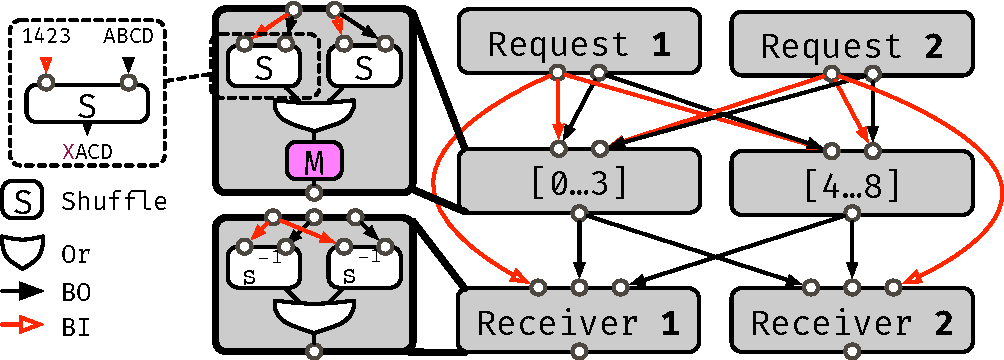
\includegraphics[width=1\columnwidth]{figs/memsplit.pdf}
  \caption{An example of splitting a memory to serve parallel requesters.}
  \label{fig:memsplit}
\end{figure}

\begin{table*}
  \centering
	\begin{tabular}{c | c | c | c}
		\textbf{Name} & \textbf{Type} & \textbf{Description} & \textbf{Definition / Default}\\\hline
		$\mathcal{N}$ & Constant & Enumeration of nodes to partition, numbered $\{n_i\}_i$ & - \\
		N & Constant, $\nnint$ & Number of operations to partition & $N = |\mathcal{N}|$\\
		P & Constant, $\nnint$ & Number of partitions to consider & $N$, or from heuristic \\
		$\mathcal{E}$ & Constant, $\{n_i \to n_j\}$& Directed edges representing dependence & - \\
		B & Variable, $\{0, 1\}^{N \times P}$ & Boolean Partitioning Matrix& - \\
		%p & Variable, $\nnint^N$ & Vector of mappings from node to assigned partition& $p = B \begin{bmatrix} 0 & 1 & \cdots & P-1\end{bmatrix}^T$\\
		$\projb{\cdot}$ & $\nnint \to \mathbb{B}$ & Function to convert a positive integer into a boolean& Supplemental Materials\\
		$\andf(\cdot, \cdot)$ & $\{0, 1\} \times \{0, 1\} \to \{0, 1\}$ & Boolean and of binary variables & Supplemental Materials \\ 
		$d_p$ & Variable, $\nnint^P$ & Vector of partition delays & - \\
		$d_n$ & Variable, $\nnint^N$ & Vector of node delays & - \\
		$\dest(n)$ & $\mathcal{N} \to \mathcal{P}(\mathcal{N})$& The set of nodes which depend on $n$& $\{n' | n' \in \mathcal{N}\ s.t.\ (n \to n') \in \mathcal{E}\}$\\
		$c_o$ & Constant, $\nnint$ & Maximum output arity of a partition & HW Spec \\
		$c_i$ & Constant, $\nnint$ & Maximum input arity of a partition & HW Spec \\
		$b_d$ & Constant, $\nnint$ & Maximum input buffer depth & HW Spec \\
		$K$ & Constant, $\mathbb{R}_+$ & Very Large Constant, used for constraint activation & $P \times N$ \\
		$\alpha_d$ & Hyperparameter, $\mathbb{R}_+$ & Retime merging probability multiplier& $\frac{1}{\max\{c_o, c_i\}}$ \\
	\end{tabular}
	\caption{Names and definitions used in the solver-based partitioning.}
	\label{tab:solver-variables}
\end{table*}

\begin{table*}
  \centering
  \newcommand\cola{1.6cm}
  \newcommand\colb{3.8cm}
  \newcommand\colc{9cm}
  \newcommand{\gcell}[2]{\Gape[#1cm][0cm]{\makecell[l]{#2}}}
  \begin{tabularx}{\textwidth}{cp{\colb}X}
    \toprule
		\textbf{Type} & \textbf{Description} & \textbf{Expression}\\\midrule
    \multirow{3}{*}{\makecell[l]{Cost\\Function}} & Allocated Partitions & $\Sigma_i \projb{\Sigma_j B_{i, j}}$\\

    & \makecell[l]{Additional Retiming\\Partitions}
    & $\alpha_d \Sigma_{n_i \to n_j \in \mathcal{E}} \projb{\max\{d_n(j) - d_n(i) - b_d, 0\}}$\\[0.3cm]
		\hline

    \multirow{12}{\cola}{\makecell[l]{\\\\Constraint}} & Partition Assignment & $ \forall n_i \in \mathcal{N}:\ \Sigma_j B_{i, j} = 1$\\[0.1cm]

    &\makecell[l]{Dependency\\Constraint} & $\forall n_i \to n_j \in \mathcal{E}:\ d_n(i) + 1[p_i \ne p_j] \le d_n(j)$\\[0.1cm]

    &\makecell[l]{Output Arity\\ Constraint} 
    &\makecell[l]{
      $\forall p \in [0, P):$ \\
      $\Sigma_{n_s \in \mathcal{N}} \andf(B_{s, p}, \projb{\max\{(\Sigma_{n_d \in \dest(n_s)} B_{d, p}) -$ \\
      $K \times B_{s, p}, 0\}}) \le c_o$
    }\\[0.7cm]

    &\makecell[l]{Input Arity Constraint\\ (vectorized)} & $\Sigma_{n_i \in \mathcal{N}} \max\{\projb{\Sigma_{n_j \in \dest(n_i)} B_{j, :}} - B_{i, :}, 0\} \le c_i \times \vec{1}$\\

		&Delay Consistency& 
    \makecell[l]{
    $\forall n_i \in \mathcal{N}:\ d_n(i) \le \min_j (d_p(j) + K - B_{i, j} \times K)$ \\
		$\forall n_i \in \mathcal{N}:\ d_n(i) \ge \max_j (d_p(j) + B_{i, j} \times K - K)$
    }\\[0.5cm]

		&Constant Validity& 
    \makecell[l]{
      $\forall n_i \in \mathcal{N}:\ d_n(i) \le K$\\
		  $\forall i \in [0, P):\ d_p(i) \le K$
    } \\
    \bottomrule
	\end{tabularx}
  \caption{Solver formulation for partitioning*.}
	\label{tab:solver-eqns}
\end{table*}

\begin{table*}
	\begin{tabular}{c | c | c | c}
		\textbf{Name} & \textbf{Type} & \textbf{Description} & \textbf{Definition / Default}\\\hline
		$\mathcal{C}_r$& $[\mathcal{N} \to \mathbb{R}_+,\mathbb{R}_+, [\mathbb{R}_+] \to \mathbb{R}_+]$ & List of per-node values, limits, and reduction& Supplemental Materials\\&& functions for reducible constraints& \\
		F & $\{0, 1\}^{N \times P}$ & Feasibility matrix, whether a partition can support a node& HW Spec \\ 
	\end{tabular}
	\caption{\Cref{tab:solver-variables} extension for solver-based merging, which is a generalization of the partitioning problem.}
	\label{tab:merging-variables}

	\begin{tabular}{c | c | c}
		\textbf{Type} & \textbf{Description} & \textbf{Expression}\\\hline
		Constraint & Feasibility Constraint & $ \forall i, j \in [0, N) \times [0, P):\ B_{i, j} \le F_{i, j}$\\
		& Reducible Constraints & $\forall j \in [0, P).\ \forall (c(\cdot), c_v, r(\cdot)) \in \mathcal{C}:\ r([c(n_i) \times B_{i, j}]_{n_i \in \mathcal{N}}) \le c_v$\\
	\end{tabular}
  \caption{\Cref{tab:solver-eqns} extension for solver-based merging*. The Retiming Partition objective is not used for merging.}
	\label{tab:merge-eqns}
  \scriptsize
  \raggedright
  \vspace{-0.3cm}
  *Expressions are presented using the Disciplined Convex Programming ruleset \cite{DCP, DCP-online}. Explanations for selected expressions can be found in the supplemental material.
\end{table*}



\name{} then set ups the crossbar data path between the parallel producers, memory partitions, and parallel consumers.
As discussed in \Cref{sec:sync}, each accessor is split into a requester actor and receiver actor.
For each memory partition, \name{} uses an actor to merge the requests from all parallel requesters, \Cref{fig:memsplit}.
The merge actor uses a special shuffle operator that shuffles the BO vector from the order in BI to the order aligned with banks in its partition.
If a bank in the partition is not accessed in BI, the output of the shuffle is marked as invalid.
We assume the capacity of each physical bank is much smaller than $2^{31}$. 
So we use the first bit of the 32-bit BO to indicate invalid accesses (0 is invalid), which is also used to explicitly disabled access from the program.
Next, the merger actor uses a tree of bit-wise OR operators to combine all bank-aligned BOs, and send the combined request vector to its partition.
The requests can be trivially ORed because static banking (\Cref{sec:background}) guarantees that no two requesters access the same bank in the same cycle.
Next, the memory partitions broadcast the respond to all receiver actors.
A receiver takes response from all partitions, using the same shuffle operators to align each response back to the requested order in BI, and uses another OR tree to merge the response. 
The BI is forwarded from the requester to the receiver for the reverse shuffling.

The alternative approach is to reverse the respond to access ordering within the memory partitions before sending them to the requester.
This approach does not scale with network bandwidth, as the memory partitions need to send the receiver number of distinct outputs.
(The number of receivers is a function of the parallelization factor.) 
As a result, the amount of output bandwidth at the memory partition limits how much the program can be parallelized, which causes underutilization of the accelerators.
In our scheme, each partition sends a single broadcast to all receivers, which is efficiently handled by the network.

The request trees for memory partition and receiver can have high fan-in, which can 
be partitioned into a tree of VB during the compute partitioning phase in \Cref{sec:compsplit}.

\subsection{Virtual Compute Decomposition} 
\label{sec:compsplit}

\subparagraph{Partitioning.}
The {\em compute-partitioning} phase addresses VBs using more compute than any PB can provide. 
If a VB contains multiple actors, \name{} first attempts to move the actors into separate VBs.
If a single actor exceeds the resource limit, \name{} breaks down the large dataflow graph in the actor into multiple actors and put them in separate VBs.
During partitioning, \name{} maps each subgraph of the large dataflow graph into a new actor, mirrors the control states of the original actor, and streams live variables in between.
The PB constraint includes the number of operations, input, and output ports available in the PBs.
Because the global network is specialized to handle efficient broadcasts, the in- and out-degree constraint counts the number of broadcast edges, as supposed to edges between partitions (\Cref{fig:parteg}(a)).
In addition, the partitioned subgraphs cannot form {\em new} cycle between partitions that did not exists in the original VGDFG. 
\Cref{fig:parteg} (b) shows an illegal partitioning that fails the cycle constraint.
This is because each actor is enabled atomically by all of its data-dependencies; cyclic dependencies between actors cause deadlock.
The original dataflow graph, however, can contain cycles that correspond to LCDs.
The back edge of the LCD is initialized with dummy data to enable execution in the first iteration.

\subparagraph{Retiming.}
To pipeline all partitions at full-throughput, \name{} must retime the imbalanced data paths between partitions with sufficient buffering. 
Retiming can introduce new VBs in addition to partitioned VBs.
The objective of this phase is to minimize the number of partitions after retiming and minimizing the amount of connectivities between partitions.

The partitioner ``fixes'' the VB based on a single PB specification, albeit there are many potential PBs the decomposed VB can be mapped to.
Currently, we use a heuristic to select a PB type from the $dom(VB)$ right before the compute pruning as a guiding constraint for partitioning.
In the following sections, we present a traversal-based solution that provides a decent solution with fast compile time, and a convex optimization solver-based solution that provides an optimum solution with long turn-around time.

\begin{figure}
  \centering
  %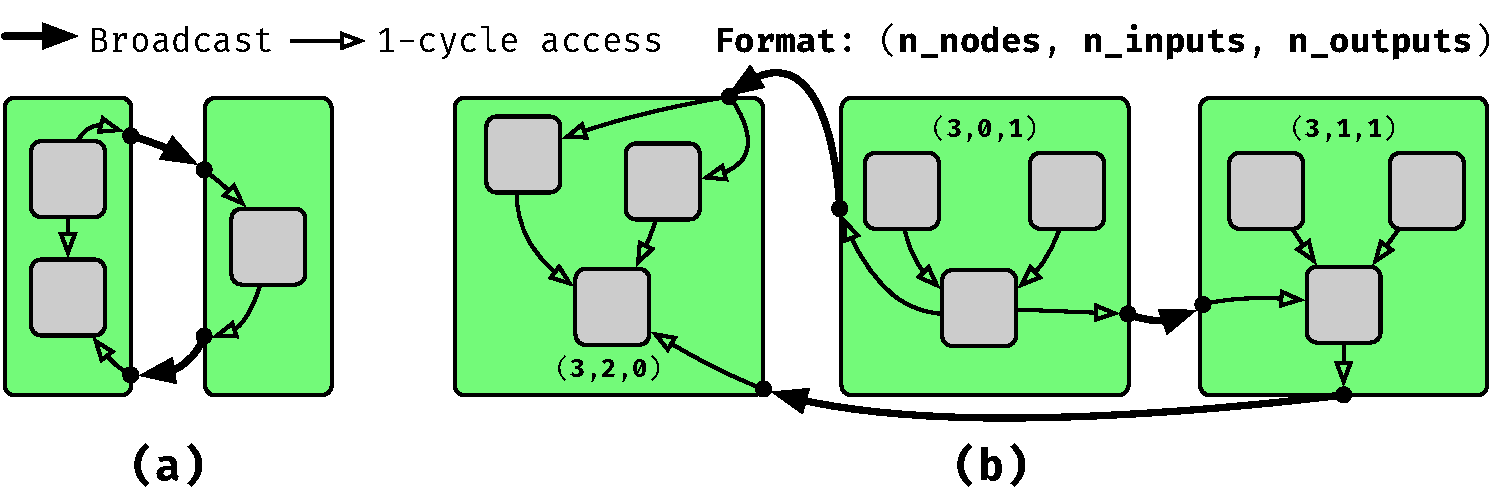
\includegraphics[width=1\columnwidth]{figs/partition_example.pdf}
  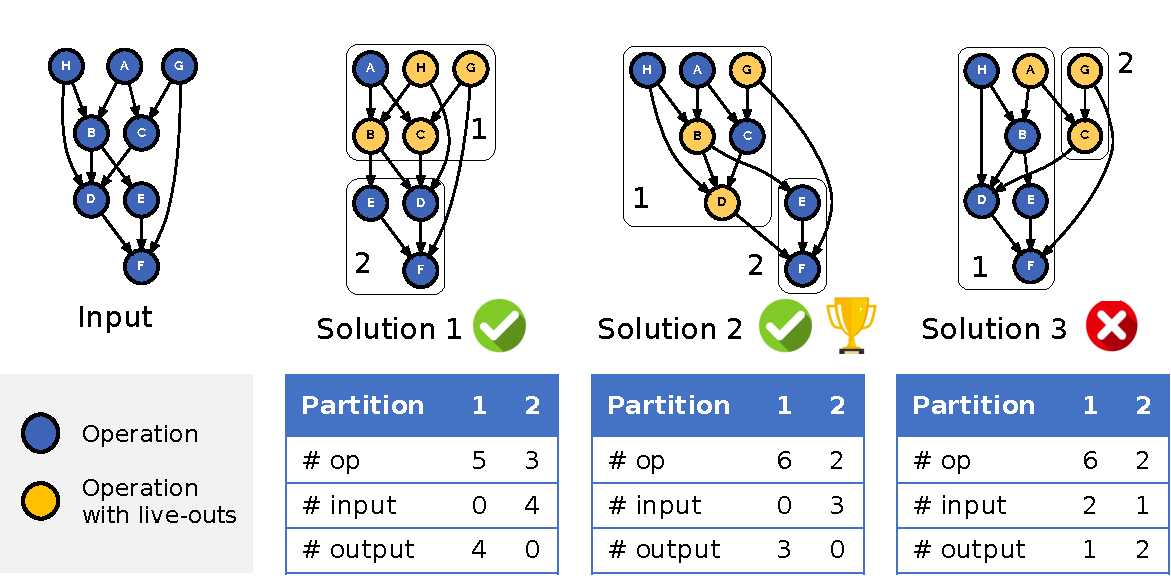
\includegraphics[width=1\columnwidth]{figs/parteg.pdf}
  \caption[Compute partitioning example]{
    \todo{}
    %(a) An example of an illegal partition. (b) The cost of a partition.
  }
  \label{fig:parteg}
\end{figure}

\paragraph{Traversal-based Solution}
To address the cycle constraint, we perform a topological sort of the dataflow graph.
The topological traversal ignores the back-edge in the graph and produces a list of traversed nodes. 
The compiler starts from the beginning of the list, recursively adds nodes into a partition until the partition no longer satisfies the hardware constraint, and repeats the process with a new partition.
This approach guarantees that no cycle is introduced with $O(V+E)$ complexity, where $V$ and $E$ are the numbers of vertices and edges.
However, the outcome of the partitioning is a function of the traversal order, which does not guarantee an optimum solution, which we experienced with depth-first search (DFS) and breadth-first search (BFS) with forwarding and backward traversals.
For DFS, we re-sort the remaining list each time we start with a new partition.

%The forward traversal schedules nodes as earlier as possible, which reduces the number of
%external live variables and the backward traversal minimizes the number of internal variables.
%The DFS minimizes the number of live variables between partitions, albeit producing more imbalanced paths between
%partitions. On the other hand, BFS produces more balanced partitioning with more live variables and partitions.

\paragraph{Solver-based Solution}
\Cref{tab:solver-eqns} gives our formulation of the partitioning problem.
At a high-level, we use a boolean matrix $B$ to keep track of the assignment of nodes in the dataflow graph to partitions. 
$B$ has dimension of number of nodes to number of partitions, where$B[i,j]==1$ indicates an assignment of node $i$ to partition $j$. 
Each node is constrained to have a single partition assignment.
The input and output arity constraints show the formulation of the PB I/O constraints.
These are the two most challenging constraints as we need to identify broadcast edges across partitions.
To address the cycle constraint, we introduce a delay vector $d$ with size equal to the number of nodes. 
The delay vector encodes a schedule to execute each node. 
A node cannot execute earlier than its input dependencies and cannot be scheduled later than its output dependencies (Delay Consistency).
The dependency constraint further limits nodes belonging to the same partition to have the same delay.
This delay variable is also used to calculate where retiming is required and projection of the amount of retiming VBs introduced. 
The final object is just the sum of partitioned VBs and retiming VBs.
To limit $B$ to a small size, we use the traversal solution to determines the initial column size of $B$.

\section{Optimizations}\label{sec:opt}
In this section, we discuss a few compiler optimizations that improve the runtime or reduces resource usage in RDAs.

\subparagraph{Memory strength reduction (msr).} Like traditional strength reduction on arithmetics, \name{} replaces expensive on-chip memories with cheaper memories whenever possible.
%We map register accumulation in the program with single-cycle initiation interval to pipeline registers.
For example, \name{} replaces a scratchpad with constant address in all accesses to a un-indexable memory, such as a FIFO.
This commonly happens when producer and consumer loops of the memory are fully unrolled.

\subparagraph{Route-Through Elimination (rtelm).} For patterns where the content of a non-indexable memory  (M1) is read and written to another memory (M2), \name{} eliminates the intermediate access if the read of M1 and the write of M2 operates in lock-step.

\subparagraph{Retiming with scratchpad (retime-mem).} By default, \name{} uses PB input buffers for retiming purpose. 
This option enables \name{} to use scratchpad memory for retiming that requires large buffer depth.

\subparagraph{Crossbar datapath elimination (xbar-elm).}
Although, crossbars between accessors and memory partitions (\Cref{sec:memsplit}) are very expensive in the general case, the BI sometimes can be statically resolvable with certain combinations of parallelization on memory accesses. 
When BI is a constant, \name{} can use this information to intelligently assign virtual banks to partitions that reduce the crossbar data path to a partial or a point-to-point connection.

\subparagraph{Read request duplication (dupra).} During memory partitioning (\Cref{sec:memsplit}), instead of forwarding BI from the requester to receiver, \name{} can also duplicate the BI with local state on receiver side, which
eliminates the unbalanced data path at the cost of extra computation.

\begin{figure*}
\centering
\begin{subfigure}[b]{0.6\textwidth}
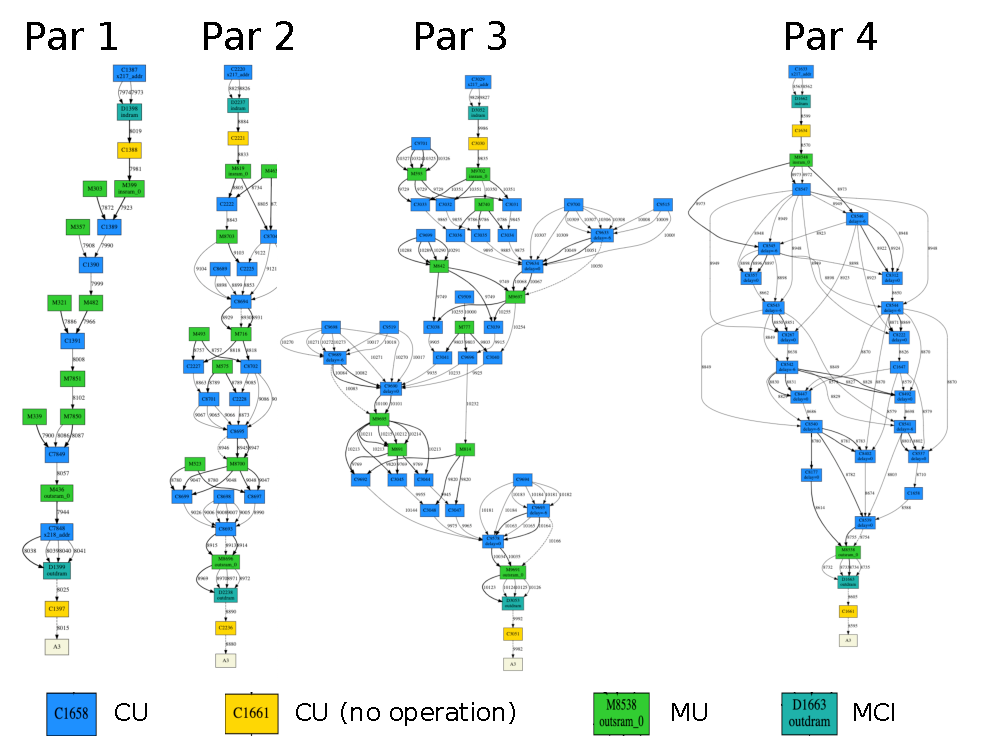
\includegraphics[width=1\textwidth]{figs/mlpunroll.pdf}
\caption{VUDFGs with different parallelization factors}
\end{subfigure}
\hfill
\begin{subfigure}[b]{0.39\textwidth}
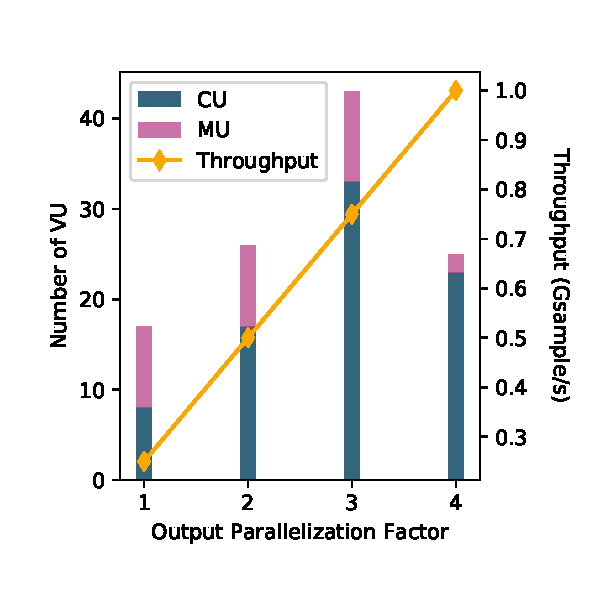
\includegraphics[width=1\textwidth]{figs/mlp.pdf}
\caption{Throughput and resource as a function of parallelization factor}
\end{subfigure}
\caption[MLP case study]{
  MLP case study
}
\label{fig:mlp}
\end{figure*}

\subparagraph{Global Merging (merge).}
After all VBs satisfy the hardware constraint, we perform a global optimization to compact small VBs into  larger VBs. 
Merging has very similar problem statement as compute partitioning (\Cref{sec:compsplit}) except with more constraints.
The traversal-based algorithm requires a reference cost for PB to check if the merged VB still satisfy the hardware constraint.
At each step of merging, we take the union of the domains of VBs within the current partition, and intersect with the domain of the merging VB.
The caveat is that even with a non-empty intersection, the bipartite graph might not have a possible assignment, as merged VB might fit in a larger PB with insufficient quantity.
Therefore, we perform a heuristic checking on feasibility of the bipartite assignment at each step of merging.
The solver-based solution combines partition assignment with PB type assignment as a joint problem. 
The output of merging gives both partition assignment as well as a PB type assignment, which eliminates the risk of un-mappable bipartite graph due to merging in the traversal-based solution.


%Many of the optimizations we perform are similar to standard compiler optimizations, such as Dead Code Elimination and
%Constant Propagation.
%Some of them, however, plays a much more important rule for CGRA due to coarse-grained nature of the architecture.
%In this section, we enumerates a few important optimizations that improves CGRA utilization.
%\subparagraph{Dead Code Elimination (DCE)} 
%We perform aggressive DCE on the VBDFG and only keeps computation that gets materialized to accelerator I/O and DRAM.
%\subparagraph{Constant Propagation}
%Aside from regular constant propagation on arithmetics, we also eliminates crossbar datapath when bank ID 
%can be statically resolved described later in \Cref{sec:memsplit}.
%During loop unrolling, address of indexable memory sometimes can be resolved to static constant.
%For a read-only RAM with constant address, we lookup their content at compile time and embed its content into registers.
%For \emph{route-through} pattern, where content of a non-indexable memory M1 is read and written to another memory M2,
%we can eliminate the intermediate write and forward the data directly to the final memory if the compiler
%can prove the read M1 and write of M2 operates in lock-step.
%We also perform constant propagation on control signals with loop-range analysis. 
%Eliminates the control signals can expose more lock-step accesses and \emph{route-through} opportunities.
%\subparagraph{Strength Reduction}
%In addition to traditional strength reduction on arithmetics, we also replace expensive memories
%with cheaper memory whenever possible.
%We map register accumulation in the program with single-cycle initiation interval to pipeline registers.
%Banked-SRAM with constant bank IDs and offsets in all accessors can also be replaced with FIFOs,
%which is happens when producer and consumer loops are fully unrolled.

%Accesses statically banked in the input graph can operates concurrently 
%without bank conflicts, as explained in \Cref{sec:background}.
%These accesses are usually from a unrolled loops. For banked accesses from the same pre-unrolled access, 
%\name first merge all requests before sending to the memory (details in \Cref{sec:memsplit}). 
%Because these accesses are from loop unrolling, they have the same program order and same dependency with other accesses.
%So the synchronization can be performed on the merged access, which prevents the amount of synchronization
%to increase with parallelism on a banked memory, as shown in \Cref{fig:mergetoken}

%\subsubsection{Blackbox IP Pruning} \label{sec:bbsplit}
%\yz{Cut this if out of the space}
%This step illustrates an example of integrating a customized partitioner for composable IP available on
%the architecture.
%The cost metrics and partition rule is specific to each IP.
%The example IP is a merge buffer, which can merge two sorted vector streams into a single stream with
%one vector per cycle throughput.
%The merge buffer pruner uses a tree of 2-way merge buffers across PBs to compose a multi-way merge buffer declared in the program.


